\tikzstyle{int} = [pin edge={to-,thin,black}]
\tikzstyle{sqr}  = [rectangle, rounded corners, minimum width=4.25cm, minimum height=1cm,text centered, draw=black, fill=white]
\tikzstyle{arrow} = [thin,->,>=stealth]

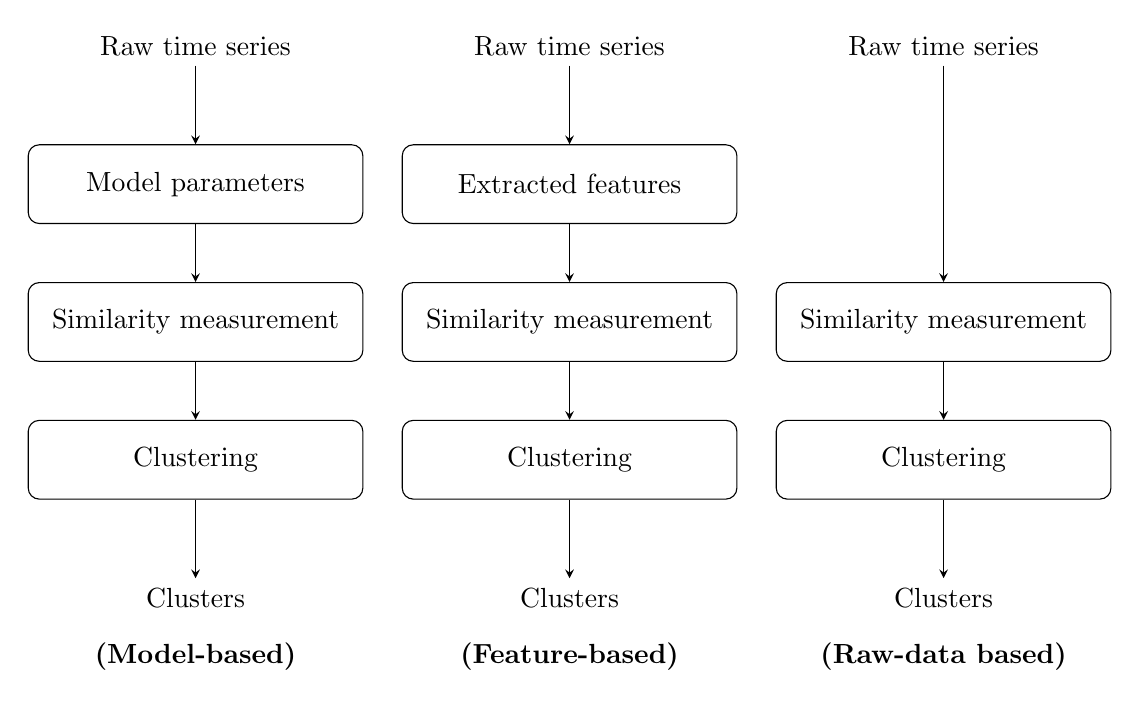
\begin{tikzpicture}[node distance=1.75cm]

%% Model-based approach
\node (inp_mod) [int] {Raw time series};
\node (rep_mod) [sqr, below of=inp_mod] {Model parameters};
\node (sim_mod) [sqr, below of=rep_mod] {Similarity measurement};
\node (clu_mod) [sqr, below of=sim_mod] {Clustering};
\node (out_mod) [int, below of=clu_mod] {Clusters};

%% Feature-based approach
\node (inp_fea) [int, right of=inp_mod, xshift=3cm] {Raw time series};
\node (rep_fea) [sqr, below of=inp_fea] {Extracted features};
\node (sim_fea) [sqr, below of=rep_fea] {Similarity measurement};
\node (clu_fea) [sqr, below of=sim_fea] {Clustering};
\node (out_fea) [int, below of=clu_fea] {Clusters};

%% Raw-data based approach
\node (inp_raw) [int, right of=inp_fea, xshift=3cm] {Raw time series};
\node (sim_raw) [sqr, right of=sim_fea, xshift=3cm] {Similarity measurement};
\node (clu_raw) [sqr, below of=sim_raw] {Clustering};
\node (out_raw) [int, below of=clu_raw] {Clusters};

%% Names
\node (nam_mod) [int, below of=out_mod, yshift=1cm] {\textbf{(Model-based)}};
\node (nam_fea) [int, below of=out_fea, yshift=1cm] {\textbf{(Feature-based)}};
\node (nam_raw) [int, below of=out_raw, yshift=1cm] {\textbf{(Raw-data based)}};

%% Arrows
\draw [arrow] (inp_mod) -- (rep_mod);
\draw [arrow] (rep_mod) -- (sim_mod);
\draw [arrow] (sim_mod) -- (clu_mod);
\draw [arrow] (clu_mod) -- (out_mod);

\draw [arrow] (inp_fea) -- (rep_fea);
\draw [arrow] (rep_fea) -- (sim_fea);
\draw [arrow] (sim_fea) -- (clu_fea);
\draw [arrow] (clu_fea) -- (out_fea);

\draw [arrow] (inp_raw) -- (sim_raw);
\draw [arrow] (sim_raw) -- (clu_raw);
\draw [arrow] (clu_raw) -- (out_raw);
\end{tikzpicture}